\section{Modelos projetados}
\subsection{Plantas}
Robôs 1 e 2

TODO: descrição do funcionamento dos robôs

\begin{figure}[H]%
  \centering
  \begin{subfigure}[b]{0.45\textwidth}
      \centering
      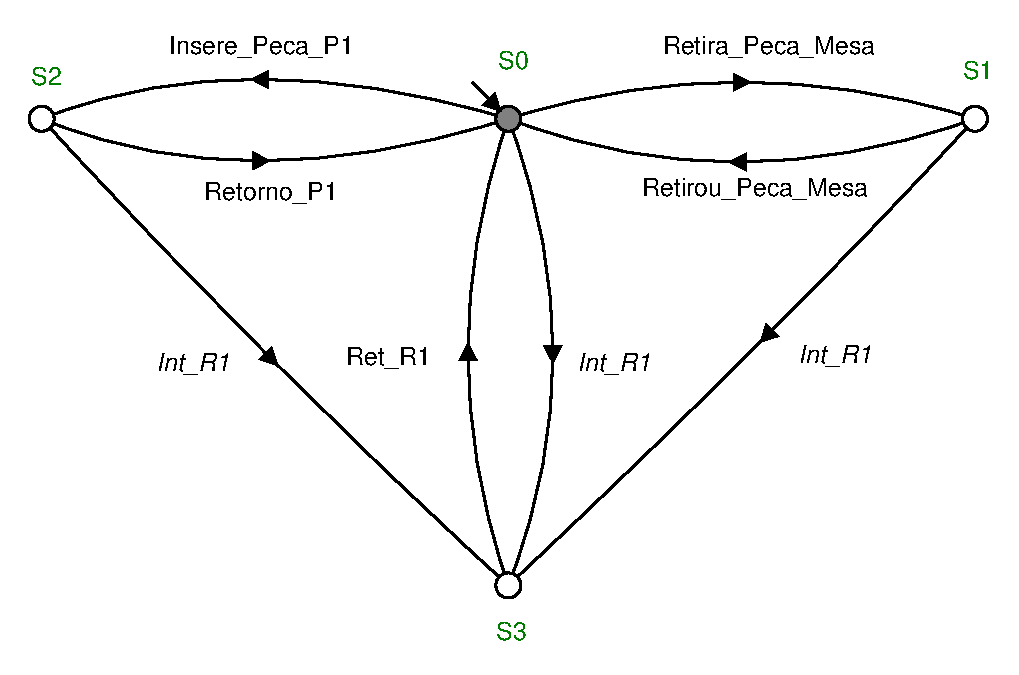
\includegraphics[width=\textwidth]{imagens/Robo_1.eps}
      \caption{Robô 1}
      \label{fig:r1}
  \end{subfigure}
  \hfill
  \begin{subfigure}[b]{0.45\textwidth}
      \centering
      \includegraphics[width=\textwidth]{imagens/Robo_2.eps}
      \caption{Robô 2}
      \label{fig:r2}
  \end{subfigure}
  \caption{Planta Robôs 1 e 2}
  \label{fig:robo12}
\end{figure}

Robôs 3 e 4

TODO: descrição do funcionamento dos robôs

\begin{figure}[H]%
  \centering
  \begin{subfigure}[b]{0.45\textwidth}
      \centering
      \includegraphics[width=\textwidth]{imagens/Robo_3.eps}
      \caption{Robô 3}
      \label{fig:r3}
  \end{subfigure}
  \hfill
  \begin{subfigure}[b]{0.45\textwidth}
      \centering
      \includegraphics[width=\textwidth]{imagens/Robo_4.eps}
      \caption{Robô 4}
      \label{fig:r4}
  \end{subfigure}
  \caption{Planta Robôs 3 e 4}
  \label{fig:robo34}
\end{figure}

Robô 5

TODO: descrição do funcionamento do robô

\begin{figure}[H]%
    \centering
    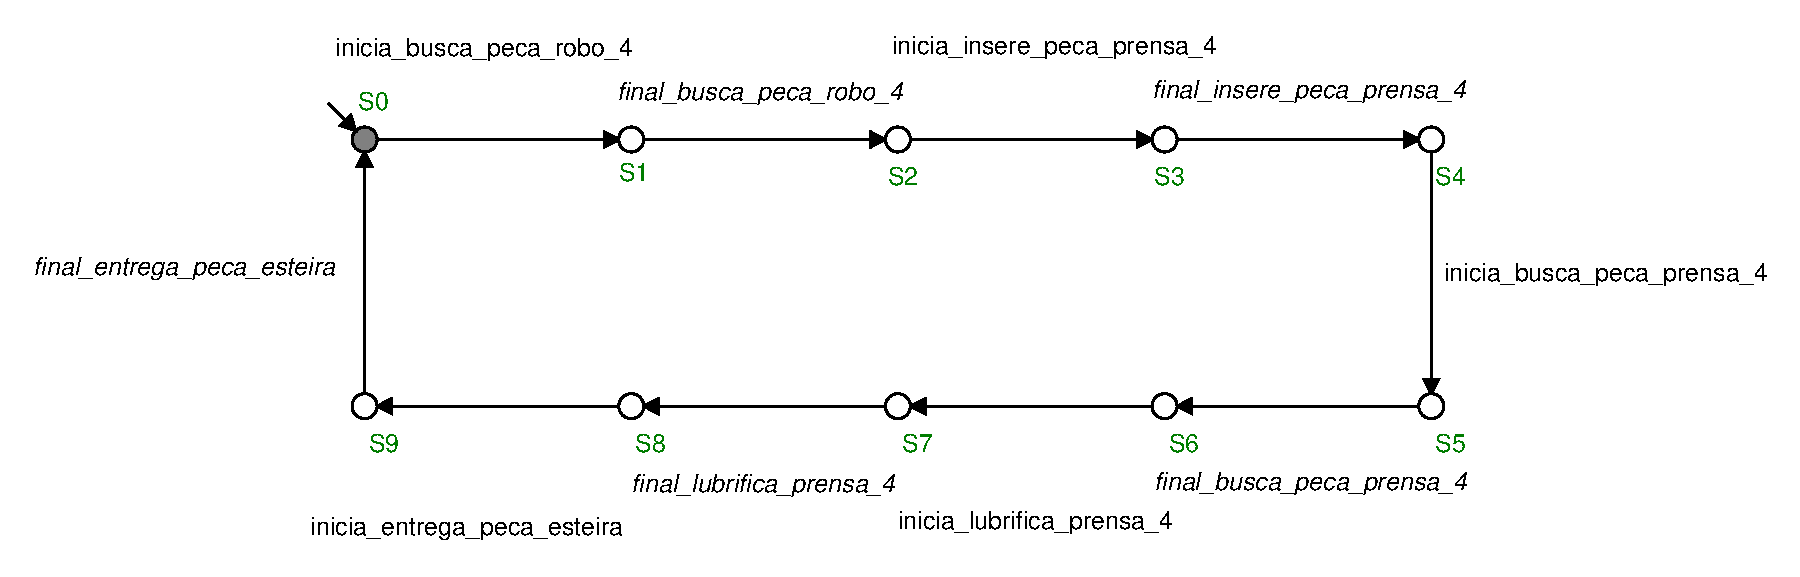
\includegraphics[width=0.9\textwidth]{imagens/robo_5.eps}
    \caption{Planta Robô 3}\label{fig:robo5}
\end{figure}

Todas as prensas têm o mesmo modelo, a seguir apresenta-se o modelo genérico para as prensas.

TODO: descrever funcionamento esperado para uma prensa.

\begin{figure}[H]%
    \centering
    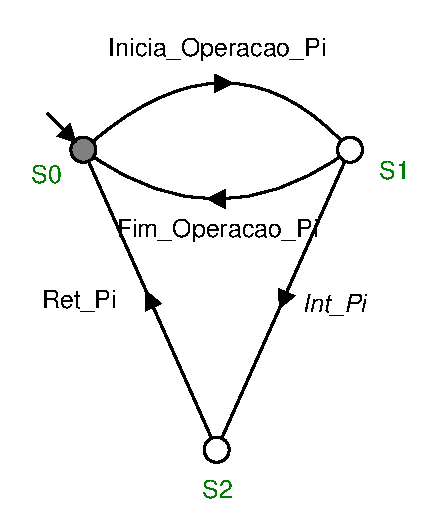
\includegraphics[width=0.6\textwidth]{imagens/Prensa.eps}
    \caption{Planta Prensa}\label{fig:prensa}
\end{figure}

\section{Especificações}
Especificação 0 inicia o processo de manufatura com a detecção de peça na mesa centralizadora.

TODO: descrição dos eventos permitidos e bloqueados

\begin{figure}[H]%
  \centering
  \begin{subfigure}[b]{0.45\textwidth}
      \centering
      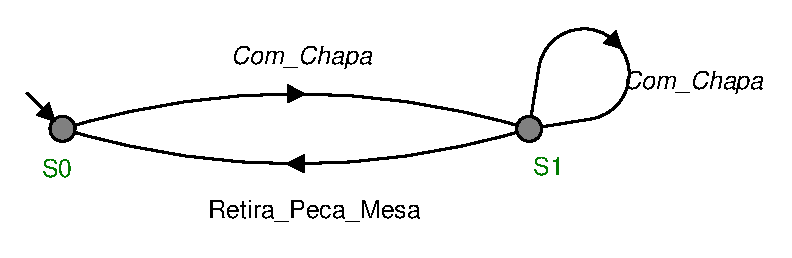
\includegraphics[width=\textwidth]{imagens/E0_inicia_R1.eps}
      \caption{Inicia R1}
      \label{fig:e0a}
  \end{subfigure}
  \hfill
  \begin{subfigure}[b]{0.45\textwidth}
      \centering
      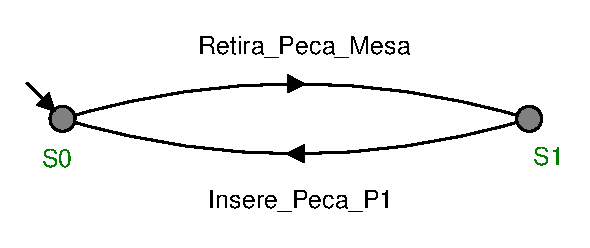
\includegraphics[width=\textwidth]{imagens/E0_finaliza_R1.eps}
      \caption{Finaliza R1}
      \label{fig:e0b}
  \end{subfigure}
  \caption{Especificação 0}
  \label{fig:e0}
\end{figure}

As especificações para início e fim das prensas são semelhantes.
Aqui será aprensentado apenas sincronização de início e fim da prensa 1, o modelo é replicado para as prensas 2, 3 e 4.

TODO: descrição de comportamento esperado de uma prensa, talvez.

\begin{figure}[H]%
  \centering
  \begin{subfigure}[b]{0.45\textwidth}
      \centering
      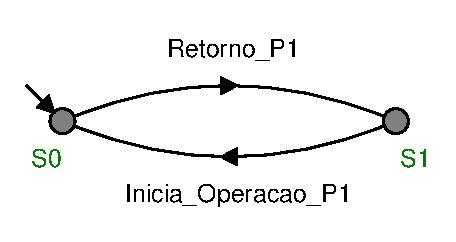
\includegraphics[width=\textwidth]{imagens/E1_inicia_P1.eps}
      \caption{Inicia P1}
      \label{fig:e1a}
  \end{subfigure}
  \hfill
  \begin{subfigure}[b]{0.45\textwidth}
      \centering
      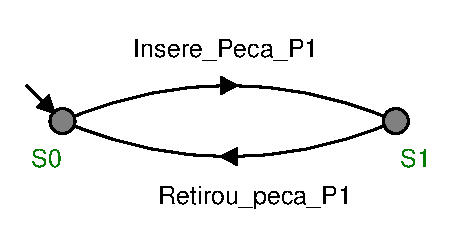
\includegraphics[width=\textwidth]{imagens/E1_finaliza_P1.eps}
      \caption{Finaliza P1}
      \label{fig:e1b}
  \end{subfigure}
  \caption{Especificação 1}
  \label{fig:e1}
\end{figure}

As especificações para sincronização dos robôs 2, 3 e 4 são semelhantes, a seguir será apresentada a sincronização do robô 2.
TODO: descrever passo a passo do funcionamento, buscar na prensa, entregar para proxima prensa.
\begin{figure}[H]%
  \centering
  \begin{subfigure}[b]{0.45\textwidth}
      \centering
      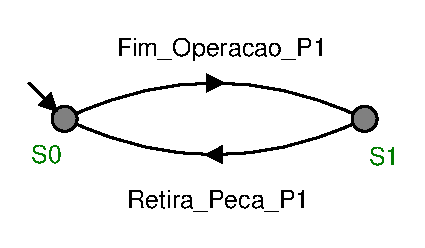
\includegraphics[width=\textwidth]{imagens/E2_inicia_R2.eps}
      \caption{Inicia R2}
      \label{fig:e2a}
  \end{subfigure}
  \hfill
  \begin{subfigure}[b]{0.45\textwidth}
      \centering
      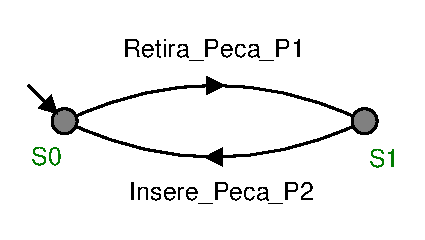
\includegraphics[width=\textwidth]{imagens/E2_Finaliza_R2.eps}
      \caption{Finaliza R2}
      \label{fig:e2b}
  \end{subfigure}
  \caption{Especificação 2}
  \label{fig:e2}
\end{figure}

O robô 5 por realizar a função de realizar a entrega da peça manufaturada em uma esteira contem especificações extras para sincronizar essa entrega.

TODO: descrição do comportamento esperado de R5 talvez

\begin{figure}[H]%
  \centering
  \begin{subfigure}{0.45\textwidth}
      \centering
      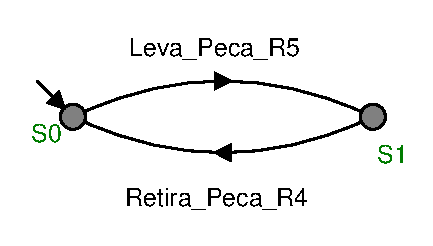
\includegraphics[width=\textwidth]{imagens/E8_inicia_R5.eps}
      \caption{Inicia busca peça de R4}
      \label{fig:e89a}
  \end{subfigure}
  \hfill
  \begin{subfigure}{0.45\textwidth}
      \centering
      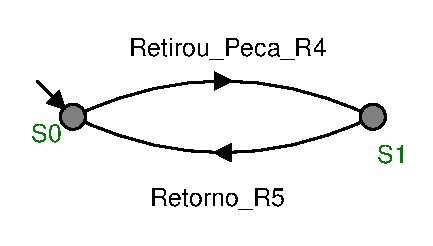
\includegraphics[width=\textwidth]{imagens/E8_finaliza_R5.eps}
      \caption{Finaliza busca peça de R4}
      \label{fig:e89b}
  \end{subfigure}
  \hfill
  \begin{subfigure}{0.45\textwidth}
      \centering
      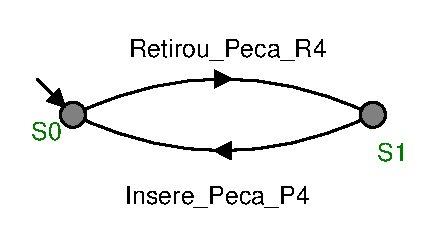
\includegraphics[width=\textwidth]{imagens/E9_inicia_entrega_P4.eps}
      \caption{Insere peça em P4}
      \label{fig:e89c}
  \end{subfigure}
  \hfill
  \begin{subfigure}{0.45\textwidth}
      \centering
      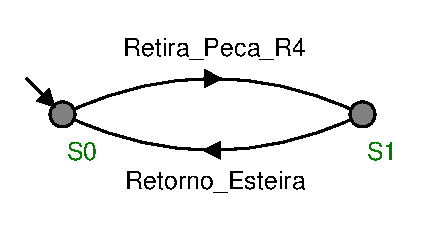
\includegraphics[width=\textwidth]{imagens/E9_finaliza_entrega_P4.eps}
      \caption{Finaliza entrega esteira}
      \label{fig:e89d}
  \end{subfigure}
  \caption{Especificação 3}
  \label{fig:e89}
\end{figure}

\section{Solução de controle modular}
TODO: descrição de qual especificação interage com quais plantas e exemplo de estrutura modular.
E0 inicia R1 interage com Robo 1 e Sensor Chapa, mas não com Prensa 1.
\begin{figure}[H]%
  \centering
  \includegraphics[width=0.8\textwidth]{imagens/modular_E0_inicia.eps}
  \caption{Planta industrial}\label{fig:modular}
\end{figure}

TODO: supervisor para cada especificação e composição de todos os supervisóes com número de estados. 